\question Ai、Bi、Ci-1分别代表被加数Ai、加数Bi和低位传来的进位,Ci代表本位向高位的进位。则下列逻辑表达式正确的是
\par\fourch{\textcolor{red}{}}{}{}{}
\begin{solution}A。 当Ai、Bi、Ci-1组成的3位二进制数中1的个数大于等于2时,Ci=1。
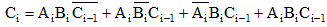
\includegraphics[width=3.40625in,height=0.28125in]{computerassets/ab8641fde06fc5054ca6997de268bf43.jpeg}
(其实就是110、101、011、111时)
详细总结可参考《计算机组成原理高分笔记》2.4节的内容。
\end{solution}
\question ALU属于
\par\twoch{时序电路}{控制器}{\textcolor{red}{组合逻辑电路}}{寄存器}
\begin{solution}C。 ALU属于组合逻辑电路。
\end{solution}
\question 算术/逻辑运算单元74181可完成
\par\twoch{16位算术运算功能}{4位乘法运算功能和除法运算功能}{16种逻辑运算功能}{\textcolor{red}{16种算术运算功能和16种逻辑运算功能}}
\begin{solution}D。
\end{solution}
\question 用4片74181和一片74182相配合,具有( )传递功能
\par\twoch{串行进位}{组内并行进位,组间串行进位}{组内串行进位,组间并行进位}{\textcolor{red}{组内、组间均为并行进位}}
\begin{solution}D。 两级分组并行进位,组内并行,组间也并行。
\end{solution}
\question 某机器有一个标志寄存器,其中有进位/借位标志CF、零标志ZF、符号标志SF和溢出标志OF,条件转移指令bgt(无符号整数比较大时转移)的转移条件是(
)
\par\fourch{}{}{\textcolor{red}{}}{}
\begin{solution}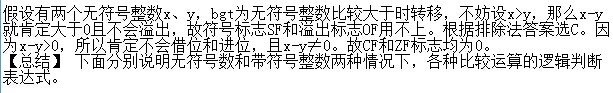
\includegraphics[width=5.72917in,height=0.86458in]{computerassets/74EF34BCDCBB2EFCE7D844D3089A1667.jpg}
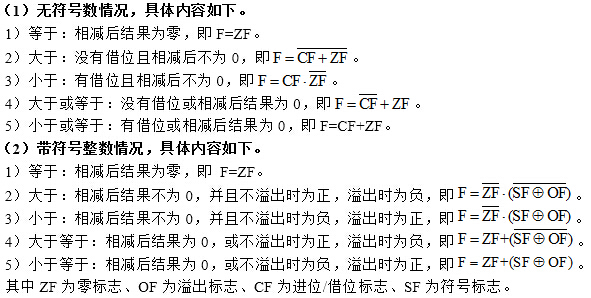
\includegraphics[width=6.15625in,height=3.10417in]{computerassets/b2a998cc87dd3475e9efee2910f922bf.jpeg}
\end{solution}
